\documentclass[12pt]{exam}

\usepackage[utf8]{inputenc}  % For UTF8 source encoding.
\usepackage{amsmath}  % For displaying math equations.
\usepackage{amsfonts} % For mathematical fonts (like \mathbb{E}!).
\usepackage{upgreek}  % For upright Greek letters, such as \upvarphi.
\usepackage{wasysym}  % For additional glyphs (like \smiley!).
\usepackage{mathrsfs} % For script text (hash families and universes).
\usepackage{enumitem}
\usepackage{graphicx}
% For document margins.
\usepackage[left=.8in, right=.8in, top=1in, bottom=1in]{geometry}
\usepackage{lastpage} % For a reference to the number of pages.
\usepackage[table,xcdraw]{xcolor}
\usepackage{pdfpages}

% TODO: Enter your name here :)
\newcommand*{\authorname}{Luis A. Perez}

\newcommand*{\duedate}{Wednesday, July 3rd}
\newcommand*{\duetime}{11:59 pm}

% Fancy headers and footers
\headrule
\firstpageheader{EE 263\\Summer 2019}{Homework 1 \\ }{Due: \duedate\\at \duetime}
\runningheader{EE 263}{Homework 1}{\authorname}
\footer{}{\footnotesize{Page \thepage\ of \pageref{LastPage}}}{}

% Exam questions.
\newcommand{\Q}[1]{\question{\large{\textbf{#1}}}}
\qformat{}  % Remove formatting from exam questions.

% Useful macro commands.
\newcommand*{\bigtheta}[1]{\Theta\left( #1 \right)}
\newcommand*{\bigo}[1]{O \left( #1 \right)}
\newcommand*{\bigomega}[1]{\Omega \left( #1 \right)}
\newcommand*{\prob}[1]{\text{Pr} \left[ #1 \right]}
\newcommand*{\ex}[1]{\text{E} \left[ #1 \right]}
\newcommand*{\var}[1]{\text{Var} \left[ #1 \right]}

\newcommand*{\norm}[1]{\left\lVert #1 \right\rVert}
\newcommand*{\HH}{\mathscr{H}}   % Family of hash functions.
\newcommand*{\UU}{\mathscr{U}}   % Universe.
\newcommand*{\eps}{\varepsilon}  % Epsilon.


% Custom formatting for problem parts.
\renewcommand{\thepartno}{\roman{partno}}
\renewcommand{\partlabel}{\thepartno.}

% Framed answers.
\newcommand{\answerbox}[1]{
\begin{framed}
\hspace{\fill}
\vspace{#1}
\end{framed}}

\printanswers

\setlength\answerlinelength{2in} \setlength\answerskip{0.3in}

\begin{document}
\title{EE 263 Homework 1}
\author{\authorname}
\date{}
\maketitle
\thispagestyle{headandfoot}
\setcounter{MaxMatrixCols}{15}

\begin{questions}
%%%%%%%%%%%%%%%%%%%%%%%%%%%%%%%%%%%
\Q{A simple control algorithm for wireless networks}

\begin{solution}
\begin{enumerate}[label=(\alph*)]
  \item We show that the power control algorithm in the problem described above can be expressed as a linear dynamical system with constant input. We begin with the equation given for the update. We have:

  \begin{align*}
    p_i(t+1) &= \alpha\gamma \frac{1}{S_i}(t) p_i(t) \tag{The given algorithm} \\
    &=  \alpha\gamma  \frac{q_i(t)}{s_i(t)} p_i(t) \tag{Definition of $S_i$} \\
    &= \alpha \gamma \frac{\sigma^2 + \sum_{j \neq i} G_{ij} p_j(t)}{G_{ii} p_i(t)} p_i(t) \tag{Definition of $s_i(t)$ and $q_i(t)$} \\
    &= \frac{\alpha \gamma \sigma^2}{G_{ii}} + \sum_{j \neq i}  (\alpha \gamma\frac{G_{ij}}{G_{ii}}) p_j(t) \tag{Distribution over sum} \\
    &= b_i + (Ap(t))_{i} \tag{Definition of matrix multiplication}
  \end{align*}
  From the above, we can easily deduce what $A \in \mathbb{R}^{n \times n}$ and $b \in \mathbb{R}^n$ should look like. We have:
  \begin{align*}
    b_i &= \frac{\alpha \gamma \sigma^2}{G_{ii}} \\
    A_{ij} &= \begin{cases}
      0 & i = j \\
      \frac{\alpha \gamma G_{ij}}{G_{ii}} & \text{otherwise}
    \end{cases}
  \end{align*}
  Note that the above is well-defined since in the problem statement $G_{ii} > 0$.
  \item We plot $S_i$ and $p_i$ as a function of $t$ in Figure \ref{fig:gamme_3_plots}, with $\gamma = 3$ and the other values as given in the problem statement. In Figure \ref{fig:gamme_5_plots}, we repeat the same process but use $\gamma = 5$.

  The observations are quite interesting. When $\gamma = 3.0$ (Figure \ref{fig:gamme_3_plots}), we see that the SINR quickly approachs our target value of $\alpha \gamma = 3.6$ (around $t = 15$). We also note that at this time, the power level for each of the three stations has stabilized.

  However, when $\gamma = 5.0$ (Figure \ref{fig:gamme_5_plots}), we see something quite different. In this case, the SINR appears to stabilize but at a value below our target. As such, the power levels of each station appear to continue to increase.

\end{enumerate}
\end{solution}

\begin{figure}[!ht]
  \centering
  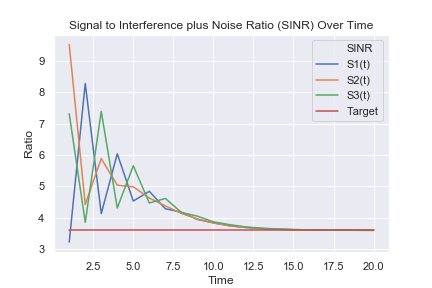
\includegraphics[scale=0.5]{figures/sinr_steps_20_gamma_3.png}
  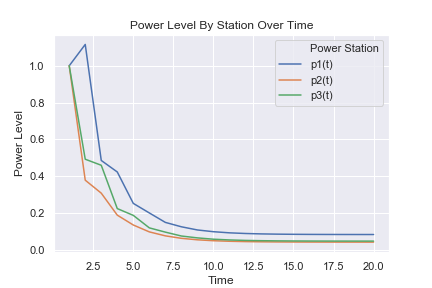
\includegraphics[scale=0.5]{figures/power_level_steps_20_gamma_3.png}
  \caption{Plot of SINR and Power Level for each of the three station over at each timestep in our simulation. We use the given parameters with $\gamma = 3.0$.}
  \label{fig:gamme_3_plots}
\end{figure}

\begin{figure}[!ht]
  \centering
  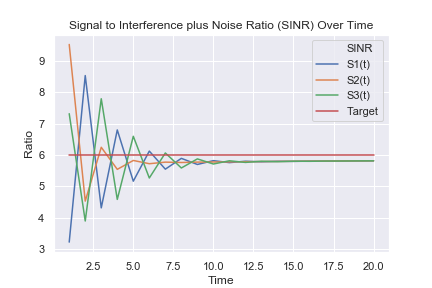
\includegraphics[scale=0.5]{figures/sinr_steps_20_gamma_5.png}
  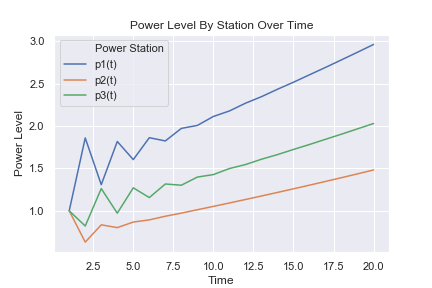
\includegraphics[scale=0.5]{figures/power_level_steps_20_gamma_5.png}
  \caption{Plot of SINR and Power Level for each of the three station over at each timestep in our simulation. We use the given parameters with $\gamma = 5.0$.}
  \label{fig:gamme_5_plots}
\end{figure}

\newpage
\Q{State equations for linear meachanical system.}

\begin{solution}
The problem gives us the definition of the linear mechanical system as:
$$
  M\ddot{q} + D\dot{q} + Kq = f
$$
where $q(t) \in \mathbb{R}^k$, $f(t) \in \mathbb{R}^k$, $M, D, K \in \mathbb{R}^{k \times k}$. Assuming $M$ is invertible, we wish to write a linear system of equations where the state $x = \begin{bmatrix} q \\ \dot{q}  \end{bmatrix} \in \mathbb{R}^{2k}$, $u = f \in \mathbb{R}^{k}$, and $y = q \in \mathbb{R}^{k}$.

The linear system of equations will therefore take the form:
\begin{align*}
  \dot{x} = Ax + Bf\\
  q = Cx + Df
\end{align*}
where $A \in \mathbb{R}^{2k \times 2k}, B \in \mathbb{R}^{2k \times k}, C \in \mathbb{R}^{k \times 2k}$ and $D \in \mathbb{R}^{k \times k}$. We also define some useful notation. Let $I_k =
  \begin{bmatrix}
    1 & 0 & \cdots  \\
    0 & 1 & \\
    \vdots &  & \ddots 
  \end{bmatrix}
\in \mathbb{R}^{k \times k}$ be the identity matrix in $\mathbb{R}^k$, and similarly, let $0_k \in \mathbb{R}^{k \times k}$ be the zero matrix in $\mathbb{R}^{k \times k}$.

The output system is the simplest. In this case, we have:
\begin{align*}
  D &= 0_k \\
  C &=
    \begin{bmatrix}
      & \vdots &  & & \vdots &\\
      \cdots & I_k & \cdots & \cdots & 0_k &  \cdots \\
       & \vdots &  & &  \vdots &
    \end{bmatrix}
  \tag{The first $k \times k$ section forms the identity matrix, and the second $k \times k$ section is all zero}
\end{align*}
With the above definitions, we have:
\begin{align*}
  y = Cx + Du &= \begin{bmatrix}
      & \vdots &  & & \vdots &\\
      \cdots & I_k & \cdots & \cdots & 0_k &  \cdots \\
       & \vdots &  & &  \vdots &
    \end{bmatrix}\begin{bmatrix} q \\ \dot{q}  \end{bmatrix} + 0_k f = q
\end{align*}
as desired.

For the dynamics equations, we first define a bit of syntax to help with notation. We note that $A \in \mathbb{R}^{2k \times 2k}$ can be divided into four equally-sized sub-matrices as follows:
$$
  A =
    \begin{bmatrix}
      A_{11} & A_{12} \\
      A_{21} & A_{22}
    \end{bmatrix}
$$
where $A_{11}, A_{12}, A_{21}, A_{22} \in \mathbb{R}^{k \times k}$. Similarly, $B$ can be decomposed in to two equally-sized matrices $B_1, B_2 \in \mathbb{R}^{k \times k}$ such that $B =
  \begin{bmatrix}
    B_1 \\
    B_2
  \end{bmatrix}$

 We then have:
\begin{align*}
  B_1 &= 0_k \\
  B_2 &= M^{-1} \\
  A_{11} &= 0_k \\
  A_{12} &= I_k \\
  A_{21} &= -M^{-1}K \\
  A_{22} &= -M^{-1}D
\end{align*}
This gives us:
\begin{align*}
  \dot{x} &= Ax + Bu  \\
  &= \begin{bmatrix}
      A_{11} & A_{12} \\
      A_{21} & A_{22}
    \end{bmatrix}
    \begin{bmatrix}
      q \\
      \dot{q}
    \end{bmatrix} +
    \begin{bmatrix}
      B_1 \\
      B_2
    \end{bmatrix}f \\
  &=
    \begin{bmatrix}
      A_{11}q + A_{12} \dot{q} \\
      A_{21}q + A_{22} \dot{q} 
    \end{bmatrix} +
    \begin{bmatrix}
      B_1f \\ 
      B_2 f
    \end{bmatrix} \\
  &= \begin{bmatrix}
    0_kq + I_k \dot{q} \\
    -M^{-1}Kq -M^{-1}D \dot{q}
    \end{bmatrix}+ 
    \begin{bmatrix}
      0_kf \\
      M^{-1} f 
    \end{bmatrix} \\
  &= \begin{bmatrix}
    \dot{q} \\
    -M^{-1}Kq -M^{-1}D\dot{q} + M^{-1} f
    \end{bmatrix} \\
  &= \begin{bmatrix}
    \dot{q} \\
    -M^{-1}(f - D\dot{q} - Kq)
    \end{bmatrix} \\
  &= \begin{bmatrix}
    \dot{q} \\
    \ddot{q}
    \end{bmatrix} \tag{As per problem statement}
\end{align*}
This shows our given linear system of equations corresponds to our mechanical system.
\end{solution}

\newpage
\Q{Some standard time-series models}

\begin{solution}
We assume the models are single-input, single-output for our discussion below. However, as the remark makes clear, the model we propose is readily extensible to multi-input, multi-output systems by allowing the referenced coefficients to be matrices (and expanding them as such in our models below).

\textbf{The MA Model}
We use the state specified in the problem statement where $x(k) =
  \begin{bmatrix}
    u(k-1) \\
    \vdots \\
     u(k-r)
  \end{bmatrix} \in \mathbb{R}^r$. We now define our matrices $A \in \mathbb{R}^{r \times r}, B \in \mathbb{R}^{r \times 1}, C \in \mathbb{R}^{1 \times r}$ and $D \in \mathbb{R}^{1 \times 1}$ as follows:
\begin{align*}
  D &=
    \begin{bmatrix}
      a_0
    \end{bmatrix} \\
  C &= 
    \begin{bmatrix}
      a_1 & \cdots & a_r
    \end{bmatrix} \\
  B &=
    \begin{bmatrix}
      1 \\
      0 \\
      \vdots \\
      0
    \end{bmatrix} \\
  A &= 
    \begin{bmatrix}
      0 & 0 & 0 & \cdots  \\
      1 & 0 & 0 & \cdots \\
      0 & 1 & 0 & \cdots \\
      0 & 0 & 1 \\
      \vdots & \vdots & \vdots & \ddots
    \end{bmatrix}
  \tag{$A_{ij} = 1$ when $i = j + 1$} 
\end{align*}
We then have:
\begin{align*}
  Ax(k) + Bu(k) &= 
  \begin{bmatrix}
      0 & 0 & 0 & \cdots  \\
      1 & 0 & 0 & \cdots \\
      0 & 1 & 0 & \cdots \\
      0 & 0 & 1 \\
      \vdots & \vdots & \vdots & \ddots
    \end{bmatrix}
  \begin{bmatrix}
    u(k-1) \\
    \vdots \\
     u(k-r)
  \end{bmatrix} + 
  \begin{bmatrix}
      1 \\
      0 \\
      \vdots \\
      0
    \end{bmatrix}
    u(k) \\
  &=
  \begin{bmatrix}
    0 \\
    u(k - 1) \\
    \vdots \\
    u(k - r + 1)
  \end{bmatrix} + 
  \begin{bmatrix}
    u(k) \\
    0 \\
    \vdots \\
  \end{bmatrix} \tag{Definition of matrix multiplication} \\
  &= \begin{bmatrix}
    u(k) \\
    u(k - 1) \\
    \vdots \\
    u(k - r + 1)
  \end{bmatrix} \tag{$A$ shifts the input down to make space for latest signal from $B$} \\
  &= x(k + 1)
\end{align*}
as desired. And also, we have:
\begin{align*}
  Cx(k) + Du(k) &=
  \begin{bmatrix}
    a_1 & \cdots & a_r
  \end{bmatrix}
  \begin{bmatrix}
    u(k-1) \\
    \vdots \\
    u(k-r)
  \end{bmatrix} + 
  \begin{bmatrix}
    a_0
  \end{bmatrix}
  u(k) \\
  & a_0 u(k) + a_1u(k-1) + \cdots a_r u(k-r) \tag{Matrix multiplication} \\
  &= y(k)
\end{align*}
which is exactly the dynamics needed for the MA model.

\textbf{The AR Model}
We use the state specified in the problem statement where $x(k) = 
  \begin{bmatrix}
    y(k-1) \\
    \vdots \\
    y(k-p)
  \end{bmatrix} \in \mathbb{R}^p$. We now define our matrices $A \in \mathbb{R}^{p \times p}, B \in \mathbb{R}^{p \times 1}, C \in \mathbb{R}^{1 \times p}$ and $D \in \mathbb{R}^{1 \times 1}$ as follows:
\begin{align*}
  D &= 
    \begin{bmatrix}
      1
    \end{bmatrix} \\
  C &=
    \begin{bmatrix}
      b_1 & \cdots & b_p
    \end{bmatrix}\\
  B &=
    \begin{bmatrix}
      1 \\
      0 \\
      \vdots
    \end{bmatrix} \\
  A &= 
    \begin{bmatrix}
      b_1 & b_2 & b_3 & \cdots  \\
      1 & 0 & 0 & \cdots \\
      0 & 1 & 0 & \cdots \\
      0 & 0 & 1 \\
      \vdots & \vdots & \vdots & \ddots
    \end{bmatrix}
  \tag{Same as $A$ for AR model except first row is filled as shown}  
\end{align*}
With the above, we have:
\begin{align*}
  Ax(k) + Bu(k) &=
    \begin{bmatrix}
      b_1 & b_2 & b_3 & \cdots  \\
      1 & 0 & 0 & \cdots \\
      0 & 1 & 0 & \cdots \\
      0 & 0 & 1 \\
      \vdots & \vdots & \vdots & \ddots
    \end{bmatrix}
    \begin{bmatrix}
      y(k-1) \\
      \vdots \\
      y(k-p)
    \end{bmatrix} + 
    \begin{bmatrix}
      1 \\
      0 \\
      \vdots
    \end{bmatrix} u(k) \\
  &= 
    \begin{bmatrix}
      b_1y(k-1) + \cdots + b_py(k-p) \\
      y(k-1) \\
      \vdots \\
      y(k-p + 1)
    \end{bmatrix} + 
    \begin{bmatrix} 
      u(k) \\
      0 \\
      \vdots
    \end{bmatrix} \\
  &=  \begin{bmatrix}
      u(k) + b_1y(k-1) + \cdots + b_py(k-p) \\
      y(k-1) \\
      \vdots \\
      y(k-p + 1)
    \end{bmatrix} \\
  &= \begin{bmatrix}
      y(k) \\
      y(k-1) \\
      \vdots \\
      y(k-p + 1)
    \end{bmatrix} \\
  &= x(k+1)
\end{align*}
The second to last line requires a bit of explanation. $A$ shifts the input down to make space for the new output. Unlike the last model where we just needed to carry the input through, in this case we need to use the input passed by $B$ ($u(k)$) to compute the current output $y(k)$. This is done by the first row of $A$ which does a weighed sum over all previous $y(k - p)$ values stored in our current state which is added to the input from $B$. It is immediate then that the new state is $x(k+1)$ as desired. 

And also, we have:
\begin{align*}
  Cx(k) + Du(k) &=
    \begin{bmatrix}
      b_1 & \cdots & b_p
    \end{bmatrix}
    \begin{bmatrix}
      y(k-1) \\
      \vdots \\
      y(k-p)
    \end{bmatrix} +
    \begin{bmatrix}
      1
    \end{bmatrix}
    u(k) \\
  &= u(k) + \sum_{i=1} b_i y(k - i) \\
  &= y(k)
\end{align*}
which is exactly the dynamics needed for the AR model.

\textbf{The ARMA Model}
We're going to do the simplest thing we can think of. We will use the state $x(k) = 
  \begin{bmatrix}
    y(k-1) \\
    \vdots \\
    y(k-p) \\
    u(k-1) \\
    \vdots \\
    u(k-r)
  \end{bmatrix} \in \mathbb{R}^{p + r}$.

This makes defining our new linear system relatively straight-forward, since we can just combine our previous two systems. We will have four matrices, $A \in \mathbb{R}^{(p+r) \times (p + r)}, B \in \mathbb{R}^{(p+r) \times 1}, C \in \mathbb{R}^{1 \times (p + r)}, D \in \mathbb{R}^{1 \times 1}$. These are defined as follows:
\begin{align*}
  D &=
    \begin{bmatrix}
      a_0
    \end{bmatrix} \\
  C &= 
    \begin{bmatrix}
      b_1 & \cdots & b_p & a_1 & \cdots & a_r
    \end{bmatrix} \\
  B &=
    \begin{bmatrix}
      a_0 \\
      0 \\
      \vdots \\
      1 \\
      0 \\
      \vdots
    \end{bmatrix} \tag{The one is at index $p + 1$} \\
    A &= 
    \begin{bmatrix}
      b_1 & b_2 & b_3 & \cdots & b_{p-1} & b_p & a_1 & a_2 & a_3 & \cdots & a_r \\
      1 & 0 & 0 & \cdots & 0 & 0 & 0 & 0 & 0 & \cdots & 0 \\
      0 & 1 & 0 & \cdots & 0 & 0 & 0 & 0 & 0 & \cdots & 0 \\
      0 & 0 & 1 & \cdots & 0 & 0 & 0 & 0 & 0 & \cdots & 0 \\
      \vdots & \vdots & \vdots & \ddots & \vdots & \vdots & \vdots & \vdots & \vdots & \vdots & \vdots \\
      0 & 0 & 0 & \cdots & 1 & 0 & 0 & 0 & 0 & \cdots & 0 \\
      0 & 0 & 0 & \cdots & 0 & 0 & 0 & 0 & 0 & \cdots & 0 \\
      0 & 0 & 0 & \cdots & 0 & 0 & 1 & 0 & 0 & \cdots & 0 \\
      0 & 0 & 0 & \cdots & 0 & 0 & 0 & 1 & 0 & \cdots & 0 \\
      0 & 0 & 0 & \cdots & 0 & 0 & 0 & 0 & 1 & \cdots & 0 \\
      \vdots & \vdots & \vdots & \vdots & \vdots & \vdots & \vdots & \vdots & \vdots & \ddots & \vdots \\
    \end{bmatrix} \tag{Note that in this case, $A_{ij} = 1$ only when $i = j + 1, j \neq p$}
\end{align*}
The above might be somewhat hard to parse, so we explain each matrix in more detail. $D$ is the same as in the MA model, since this model is idential to the MA model in that regard. $C$ is simply the concatenation of the corresponding $C$ matrices used in the AR and MA models, since the output of this model is nearly a sum of the output of both models ($D$ handles the edge-case).

The matrix $B$ perform two key purposes. It scales the input by $a_0$ so it can be used to compute the current timesteps' output (needed to generate the next state), and also simply passes the input as-is along the $p+1$ index, so it can be added to the new state.

The matrix $A$ is likely the most complicated to understand, but again, this is simply composed of four smaller submatrices. The bottom-left matrix  of dimension $r \times p$ is just all zero. The top-left matrix of dimensions $p \times p$ is the exact same as the matrix in the AR model. The bottom-right matrix of dimensions $r \times r$ is the exact same as the matrix in the MA model. And finally, the top-right matrix of dimension $p \times r$ is simply a zero matrix where the first row contains the $a_i$ co-efficients. Putting it all together, the only interesting aspect is the first row, which contains all relevant co-efficients needed to compute the current timestep's output.

As such, we have:
\begin{align*}
  Ax(k) + Bu(k) &= 
    \begin{bmatrix}
      b_1 & b_2 & b_3 & \cdots & b_{p-1} & b_p & a_1 & a_2 & a_3 & \cdots & a_r \\
      1 & 0 & 0 & \cdots & 0 & 0 & 0 & 0 & 0 & \cdots & 0 \\
      0 & 1 & 0 & \cdots & 0 & 0 & 0 & 0 & 0 & \cdots & 0 \\
      0 & 0 & 1 & \cdots & 0 & 0 & 0 & 0 & 0 & \cdots & 0 \\
      \vdots & \vdots & \vdots & \ddots & \vdots & \vdots & \vdots & \vdots & \vdots & \vdots & \vdots \\
      0 & 0 & 0 & \cdots & 1 & 0 & 0 & 0 & 0 & \cdots & 0 \\
      0 & 0 & 0 & \cdots & 0 & 0 & 0 & 0 & 0 & \cdots & 0 \\
      0 & 0 & 0 & \cdots & 0 & 0 & 1 & 0 & 0 & \cdots & 0 \\
      0 & 0 & 0 & \cdots & 0 & 0 & 0 & 1 & 0 & \cdots & 0 \\
      0 & 0 & 0 & \cdots & 0 & 0 & 0 & 0 & 1 & \cdots & 0 \\
      \vdots & \vdots & \vdots & \vdots & \vdots & \vdots & \vdots & \vdots & \vdots & \ddots & \vdots \\
    \end{bmatrix}
    \begin{bmatrix}
      y(k-1) \\
      \vdots \\
      y(k-p) \\
      u(k-1) \\
      \vdots \\
      u(k-r)
    \end{bmatrix} + 
    \begin{bmatrix}
      a_0 \\
      0 \\
      \vdots \\
      1 \\
      0 \\
      \vdots
    \end{bmatrix} u(k) \\
  &=
    \begin{bmatrix}
      b_1y(k-1) + \cdots + b_py(k-p) + a_1u(k-1) + \cdots + a_r u(k-r) \\
      y(k-1) \\ 
      \vdots \\
      y(k-p + 1) \\
      0 \\
      u(k-1) \\
      \vdots \\
      u(k - r + 1)
    \end{bmatrix}  + 
    \begin{bmatrix}
    a_0u(k) \\
    0 \\
    \vdots \\
    0 \\
    u(k) \\
    0 \\
    \vdots \\
    0
    \end{bmatrix} \\
  &=
    \begin{bmatrix}
      b_1y(k-1) + \cdots + b_py(k-p) + a_0u(k) + a_1u(k-1) + \cdots + a_r u(k-r) \\
      y(k-1) \\ 
      \vdots \\
      y(k-p + 1) \\
      u(k) \\
      u(k-1) \\
      \vdots \\
      u(k - r + 1)
    \end{bmatrix}  \\
    &=
    \begin{bmatrix}
      y(k) \\
      y(k-1) \\ 
      \vdots \\
      y(k-p + 1) \\
      u(k) \\
      u(k-1) \\
      \vdots \\
      u(k - r + 1)
    \end{bmatrix} \\
    &= x(k+1)
\end{align*}

Finally, we have:
\begin{align*}
  Cx(k) + Du(k) &=
  \begin{bmatrix}
    b_1 & \cdots & b_p & a_1 & \cdots & a_r
  \end{bmatrix}
  \begin{bmatrix}
    y(k-1) \\
    \vdots \\
    y(k-p) \\
    u(k-1) \\
    \vdots \\
    u(k-r)
  \end{bmatrix} + 
  \begin{bmatrix}
    a_0
  \end{bmatrix}u(k) \\
  &= \sum_{i=1}^{p} b_i y(k-i) + \sum_{i = 1}^{r} a_{i}u(k - i) + a_0 u(k) \\
  &= y(k)
\end{align*}
Therefore, this linear system is appropriate for the ARMA model.
\end{solution}

\newpage
\Q{Representing linear functions as matrix multiplication}

\begin{solution}
Let $f : \mathbb{R}^n \to \mathbb{R}^m$ be a linear function. We show that there is a matrix $A \in \mathbb{R}^{m \times n}$ such that for all $x \in \mathbb{R}^n, f(x) = Ax$.

To do this, we begin with some notation. Let $e_i \in \mathbb{R}^n$ be the vector containing a $1$ for the $i$-th dimension, and zero otherwise. Now, define $A$ as follows:

\begin{align*}
A_{ij} &= f(e_j)_i \tag{The $ij$-th entry of $A$ is the $i$-th entry of the result of $f(e_j)$}
\end{align*}
Stated another way, the $n$ columns of $A$ consist of $f$ evaluated on each unit basis vector.

We now show that with this $A$, we indeed have $f(x) = Ax$ for all $x \in \mathbb{R}^n$. Let us first evaluate the LHS of this equation.
\begin{align*}
f(x) &= f(x_1 e_1 + \cdots + x_n e_n) \tag{Decompose any $x$ as a linear combination of basis vectors $e_j$} \\
&= x_1f(e_1) + \cdots + x_nf(e_n) \tag{Linearity of $f$}
\end{align*}
We now evaluated the RHS. Let $A_k$ correspond to the $k$-th column of $A$.
\begin{align*}
  Ax &= x_1 A_1 + x_2 A_2 + \cdots + x_n A_n \tag{Defintion of matrix multiplication as a linear combination of matrix columns} \\
  &= x_1f(e_1) + x_2f(e_2) + \cdots + x_n f(e_n) \tag{Construction of $A$ as described above}
\end{align*}
From the above, we see that the LHS and RHS are equivalent for arbitrary choice of $x \in \mathbb{R}^n$. 

The next question is whether $A$ is unique. The answer is yes. We prove by contradiction. 

Let us suppose that a matrix $\tilde{A}$ satisfying the above properties exists, and that $\tilde{A} \neq A$.

However, by our assumption, $\tilde{A} \neq A$, so there is some $A_{ij} \neq \tilde{A}_{ij}$. As such, we have that $A_j \neq \tilde{A}_j$ (the $j$-th columns differ). Now take $x = e_j$ (the unit vector with a $1$ in the $j$-th dimension, zero everywhere else).

Then note that:
$$
f(e_j) = Ae_j = A_j \neq \tilde{A}_j = \bar{A}e_j \implies  f(e_j) \neq \bar{A}e_j
$$
This is a contradiction on the fact that $f(x) = \tilde{A}x$ for all $x \in \mathbb{R}^n$. As such, our assumption that $A \neq \bar{A}$ must be wrong.
\end{solution}

\newpage
\Q{Counting sequences in language code}
\begin{solution}
  \begin{enumerate}[label=(\alph*)]
    \item
      $B_{ij} = A^r_{ij}$ is simply the number of valid sequences in our language of length $(r+1)$ whose first symbol is $j$ and whose last symbol is $i$.

      We now proof the above claim using induction.

      \textbf{Base Case}
      For the base case, we take $r = 1$. so we have $B = A$. As given in the problem statement, $A_{ij} = 1$ if symbol $i$ is allowed to follow symbol $j$. As such, $B_{ij}$ is $1$ when the 2-letter sequence $ji$ is a valid sequence in our language. This satisfies our property, since $B_{ij}$ is then exactly the count of valid sequences of length $2$ whose first symbol is $j$ and last symbol is $i$.

      \textbf{Inductive Step}
      Suppose our property holds for $B'_{ij} = A^r$. We now show that it also holds for $B_{ij} = A^{r+1}$. To do this, we consider how to compute $B_{ij}$. This is mechanically given as:
      \begin{align*}
        B_{ij} &= A^{r+1}_{ij} \\
        &= (A A^{r})_{ij} \\
        &= (A B')_{ij} \\
        &= \sum_{k} A_{ik}B'_{kj} 
      \end{align*}
      We know that $A_{ik}$ will be $1$ if $i$ is allowed to follow $k$. By our inductive hypothesis, we know that $B'_{kj}$ is the number of valid sequences in our language of length $(r + 1)$ whose first symbol is $j$ and whose last symbol is $k$. 

      As such, the summation above will simply sum together the count of all sequence of length $(r+1)$ which start with $j$ (can end with anything) and can be extended by adding $i$ to the end. The result is therefore just the number of sequences in our language of length $(r+ 2)$ which start with $j$ and end with $i$. This proof our inductive case.

    \item 
      To solve this problem, we define $A$ as described above. In particular, we have:
      $$
      A = \begin{bmatrix}
        0 & 0 & 1 & 0 & 1 \\
        1 & 1 & 0 & 1 & 0 \\
        1 & 0 & 0 & 0 & 1 \\
        0 & 0 & 0 & 1 & 0 \\
        0 & 1 & 0 & 1 & 0
      \end{bmatrix}
      $$
      We then compute $A^9$, which turns out to be:
      $$
      A^9 = \begin{bmatrix}
        41 & 49 & 24 & 113 & 37 \\
        55 & 65 & 31 & 150 & 49 \\
        42 & 49 & 23 & 113 & 37 \\
        0 & 0 & 0 & 1 & 0 \\
        31 & 37 & 18 & 86 & 28
      \end{bmatrix}
      $$
      The above matrix contains the count of all valid words of length $10$ which begin and end with symbols $j$ and $i$. As such, just taking the sum of all entries will give us the total number of valid sequences of length $10$. This comes out to be $1079$.

      We could follow a similar approach (with $A$ being a matrix of all $1$s) to count all possible sequences of length $10$ (where all characters are allowed). However, a simpler approach is simply to compute $5^{10} = 9,765,625$. This is because we have $10$ spaces, and each space can contain any of the $5$ symbols and still be valid.

      As far as comparison, our set of valid sequences is actually very small. It is only about $0.01104896\%$.

    \item
      We wish to count, among all allowed sequences of length $10$, what the most common value for the seventh symbol is. We can do this by noting that all allowed sequences of length $10$ must consist of an allowed sequence of length $7$ which overlaps by one character with an allowed sequence of length $4$. For example, $125312$ (allowed sequence of length $7$) and $2512$ (allowed sequence of length $4$) when put together (with the final and first characters overlapping) form the sequence $12531\textbf{2}512$ of length $10$.

      With this insight, what we can do is look at the matrix $A^6$ as well as the matrix $A^4$. We know that $A^6_{ij}$ gives us the number of valid sequences in our languages of length $7$ whose first symbol is $j$ and whose last symbol is $i$. Similarly for $A^3_ki$, which gives us the number of valid sequences of length $4$ whose first symbol is $i$ and last symbol is $k$.

      Then we can define:
      $$
        Z = \left(A^6  \begin{bmatrix} 1 \\ \vdots \\ 1\end{bmatrix}\right) \times \left(\begin{bmatrix} 1 & \cdots & 1 \end{bmatrix} A^3\right)^T
      $$
      where $\times$ is element-wise multiplication.
      Then note that with the above, we have:
      \begin{align*}
        Z_i &= \sum_{j} A^6_{ij} \times  \sum_{k} A^3_{ki}
      \end{align*}
      Note that the first term in the product is counting the number of valid sequences of length $7$ which end with $i$, while the second term is counting the number of valid sequences of length $4$ which start which start with $i$. As such, $Z_i$ is simply the number of valid sequences of length $10$ which contain $i$ as their seventh symbol.

      Computing this using Python, we have:
      $$
        Z = \begin{bmatrix}
          288 \\
          446 \\
          144 \\
          14 \\
          185 \end{bmatrix}
      $$
      and from this, we can immediately determine that among all allowed sequences of length $10$, the most common value for the $7$-th symbol is $2$.
  \end{enumerate}
\end{solution}

\newpage
\Q{Express the following statements in matrix language}

\begin{solution}
\begin{enumerate}[label=(\alph*)]
  \item
    $Z = TY$ where $T_{ij} = 0$ for $i > j$ and all $i > n$. Note that the last requirement is required since the problem does not specify that $Y$ has at most $n$ rows (and as such, could have more, which must be ignored when forming $Z$).
  \item
    $W = VP$ where $P$ is a square of all zeros except near the main diagonal. There, we have small $2 \times 2$ matrices along the main diagonal. Each small $2 \times 2$ matrix is zero everywhere except the anti-diagonal (top right and bottom left) where it has ones. If the dimension of $P$ is odd, the bottom-right corner has a $1$ (we assume that in the case of an odd number of columns, the last column is left unmodified).
  \item 
    We assume the angle measured is the smallest possible angle between the two vectors (eg, $\theta' = \min\{\theta, 360^{\circ} - \theta \}$). Then we have $P^TQ = R$ where $R_{ij} \geq 0$ for all $i,j$.
  \item
    Similarly to above, we assume the angle being measured is the smallest possible angle between the two vectors. Then we have $P^TQ = R$ where $R_{ii} \geq 0$.

  \item
    $A^T A = X$ where $X_{ij} = 0$ for $i = 1, \cdots k$ and $j > k$ or $j = 1, \cdots k$ and $i > k$.

\end{enumerate}
\end{solution}

\newpage
\Q{Proof of the Cauchy-Schwarz inquality}

\begin{solution}
The proof is rather straight forward with the given hint. We show the step-by-step process below.

\begin{align*}
  || (||y|| x \pm ||x|| y) ||^2 \geq 0 \tag{Square of a real number is non-negative} \\
  \implies \sum_i (||y|| x_i \pm ||x|| y_i)^2 &\geq 0 \tag{Definition of vector norm} \\
  \implies \sum_i (||y||^2 x_i^2 + ||x||^2 y_i^2 \pm 2||x||\cdot||y||x_i y_i &\geq 0 \tag{Squaring inner sum term} \\
  \implies ||y||^2 \sum_i x_i^2 + ||x||^2 \sum_i y_i^2 \pm 2||x||\cdot||y|| \sum_i x_i y_i &\geq 0 \tag{Distributing the sum} \\
  \implies ||y||^2 ||x||^2 + ||x||^2 ||y||^2 \pm 2||x||\cdot||y|| x^Ty &\geq 0 \tag{Definition of vector norm and dot product} \\
  \implies 2 ||x||^2 ||y||^2 \geq \mp 2||x|| \cdot ||y|| x^Ty \tag{Some algebra}\\
  \implies ||x|| \cdot ||y|| \geq \mp x^T y \tag{When $||x|| \neq 0$ and $||y|| \neq 0$}
\end{align*}
As such, we have $x^Ty \leq ||x|| \cdot ||y||$ and also $x^T y \geq - ||x|| \cdot ||y||$ as long as $$||x|| \neq 0, ||y|| \neq 0$$. In the case where either vector is the zero vector, it's immediately clear that $|x^T y| = ||x || \cdot ||y||$. As such, putting all of the above together, we arrive at the Cauchy-Schwarz inequality for all $x,y$:
$$
\implies |x^Ty| \leq ||x|| \cdot ||y||
$$

As for when equality holds, the first case is when at least one of $x$ or $y$ is the zero vector. This is immediate from the definition of the inequality.

In the case where neither is the zero vector, we must have:
\begin{align*}
  |x^T y| &= ||x || \cdot ||y||\\
  \implies |\left(\frac{x^T}{||x||} \right)\left(\frac{y}{||y||} \right)| &= 1 \tag{Neither $x$ nor $y$ is the zero vector} \\
  \implies |u_x^T u_y| = 1 \tag{$u_v$ is the unit vector in the direction of $v$}
\end{align*}
The above implies that the equality holds when neither $x$ nor $y$ are the zero vector if and only if they are pointing in the same ($=1$) or opposite ($= -1$) directions.

\end{solution}

\end{questions}


\includepdf[
    %% Include all pages of the PDF
    pages=-,
    %% make this page have the usual page style
    %% (you can change it to plain etc). By default pdfpages
    %% sets the pagecommand to \pagestyle{empty}
    pagecommand={\pagestyle{headings}}]
%% The pdf file itself
{code.pdf}























\end{document}
